\section*{Введение}
Алгоритм в задаче о Ханойской башне находит последовательность действий, чтобы
переместить диски с одной башни на другую, ограничиваясь правилами игры.

Актуальность данной темы средняя, так как очень мало применений, кроме как
образовательных. Программистам-новичкам с помощью данной задачи легко
показать как работает рекурсия. Рекурсия очень важна в компьютерных
науках, ведь только с помощью рекурсии можно строго математически
перейти к процедурному-императивному циклу. Зачастую рекурсивные задачи
выглядят элегантно и красиво, что даёт особой шарм, при написании такого
кода.

Цель: реализовать графическое приложение с алгоритмами решения задачи о
Ханойское башне рекурсивным и итеративным алгоритмами на динамически
типизированном языке программирования Python\cite{Python}.

Задачи:
\begin{itemize}
	\item Научиться решать задачу о Ханойской башне
	\item Сделать графический интерфейс для игры в этот пазл
	\item Вся реализация должна быть на языке программирования Python
	\item Написать юнит-тесты для библиотеки
\end{itemize}
\addcontentsline{toc}{section}{Введение}
\section{Ханойская башня}
Ханойская башня (также называемая проблемой храма Бенареса или Башней
Брахмы или башней Лукаса, а иногда во множественном числе как Башни, или
просто пирамидальная головоломка) --- математическая игра или головоломка,
состоящая из трех стержней и нескольких дисков различного диаметра,
которые могут перемещаться по любому стержню. Головоломка начинается с того, что
диски укладываются на один стержень в порядке уменьшения размера, наименьший
вверху, таким образом, приближаясь к конической форме. Цель головоломки ---
переместить всю стопку до последнего стержня, соблюдая следующие правила:

\begin{enumerate}
	\item Одновременно можно перемещать только один диск.
	\item Каждый ход состоит в том, чтобы взять верхний диск из одной из стопок
	      и поместить его поверх другой стопки или на пустой стержень.
	\item Ни один диск не может быть помещен поверх диска, который меньше его.
\end{enumerate}

Имея 3 диска, головоломку можно решить за 7 ходов. Минимальное количество
ходов, необходимых для решения головоломки Ханойской башни, равно $2n - 1$,
где $n$ --- количество дисков.

Загадка была представлена на Западе французским математиком Эдуардом Лукасом в
1883 году. Почти сразу же всплыли\cite{book:2211323} многочисленные мифы о
древней и мистической природе головоломки, в том числе об индийском храме в
Каши Вишванатхе, в котором находится большая комната с тремя потертыми от
времени столбами, окруженными 64 золотыми дисками. Исполняя повеление древнего
пророчества, священники-брахманы с тех пор передвигают эти диски в соответствии
с непреложными правилами Брахмы. Поэтому головоломка также известна как Башня
Брахмы. Согласно легенде, когда будет выполнен последний ход головоломки,
наступит конец света.\cite{book:73336}

Если бы легенда была правдой, и если бы священники могли перемещать диски со
скоростью один в секунду, используя наименьшее количество ходов, им
потребовалось бы $2^{64}-1$ секунды или примерно 585 миллиардов лет, чтобы
закончить, что примерно в 42 раза превышает нынешний возраст вселенной.

Существует множество вариаций этой легенды. Например, в некоторых рассказах
храм --- это монастырь, а священники --- монахи. Храм или монастырь могут
находиться в разных местах, включая Ханой, и могут быть связаны с любой
религией. В некоторых версиях вводятся другие элементы, например, тот факт, что
башня была создана в начале мира, или что священники или монахи могут совершать
только один ход в день.

На текущий момент Ханойские башни используются в играх-головоломках. В
образовательных целях данная задача даётся как пример элегантного рекурсивного
решения. Можно найти веб-сайты, которые представляют собой игру в Ханойскую
башню.

\subsection{Решение}

В головоломку можно играть с любым количеством дисков, хотя во многих
игрушечных версиях их от 7 до 9. Минимальное количество ходов, необходимых для
решения головоломки Ханойской башни, равно $2n-1$, где $n$ --- количество
дисков.\cite{book:781890}

\subsubsection{Итеративное решение}

Простое решение игрушечной головоломки состоит в том, чтобы чередовать ходы
между самым маленьким и не самым маленьким фрагментами. Перемещая самую
маленькую фигуру, всегда перемещайте ее на следующую позицию в том же
направлении (вправо, если начальное количество фигур четное, влево, если
начальное количество фигур нечетное). Если в выбранном направлении нет позиции
башни, переместите фигуру в противоположный конец, но затем продолжайте
двигаться в правильном направлении. Например, если вы начали с трех фигур, вы
должны переместить самую маленькую фигуру в противоположный конец, а затем
продолжить движение в левом направлении после этого. Когда наступает очередь
переместить немаленькую фигуру, остается только один допустимый ход. Выполнение
этого алгоритма позволит завершить головоломку за наименьшее количество ходов.

\subsubsection*{Более простая формулировка итеративного решения}

Для четного числа дисков:

\begin{itemize}
	\item сделайте законный ход между колышками A и B (в любом направлении),
	\item сделайте законный ход между колышками A и C (в любом направлении),
	\item сделайте законный ход между колышками B и C (в любом направлении),
	\item повторяйте до завершения.
\end{itemize}

Для нечетного числа дисков:

\begin{itemize}
	\item сделайте законный ход между колышками A и C (в любом направлении),
	\item сделайте законный ход между колышками A и B (в любом направлении),
	\item сделайте законный ход между колышками B и C (в любом направлении),
	\item повторяйте до завершения.
\end{itemize}

В каждом случае делается в общей сложности $2n - 1$ хода.

\subsubsection{Рекурсивное решение}

Ключом к рекурсивному решению проблемы является признание того, что ее можно
разбить на набор более мелких подзадач, к каждой из которых применяется та же
общая процедура решения, которую мы ищем, и затем общее решение находится
каким-то простым способом из решений этих подзадач. Каждая из этих созданных
подзадач, будучи ``меньшей'', гарантирует, что базовый вариант (варианты) в
конечном итоге будут достигнуты:

\begin{itemize}
	\item обозначьте колышки A, B, C,
	\item пусть $n$ --- общее количество дисков,
	\item пронумеруйте диски от 1 (самый маленький, самый верхний) до $n$ (самый
	      большой, самый нижний).
\end{itemize}

Предполагая, что все n дисков распределены между колышками в правильном
порядке; предполагая, что на исходном колышке имеется m верхних дисков, а все
остальные диски больше m, поэтому их можно безопасно игнорировать; чтобы
переместить m дисков с исходного колышка на целевой колышек с помощью запасного
колышка, без нарушения правил:

\begin{enumerate}
	\item Переместите диски $m - 1$ от источника к запасному стержню, используя ту
	      же общую процедуру решения. Правила не нарушаются, по предположению. Это
	      оставляет диск m в качестве верхнего диска на исходном колышке.
	\item Переместите диск m от источника к целевому стержню, что гарантированно
	      является допустимым ходом, по предположениям — простой шаг.
	\item Переместите диски $m - 1$, которые мы только что поместили на запасной, с
	      запасного на целевой колышек с помощью той же общей процедуры решения,
	      чтобы они были размещены поверх диска m без нарушения правил.
	\item Базовый вариант – переместить 0 дисков (на этапах 1 и 3), то есть
	      ничего не делать, что, очевидно, не нарушает правила.
\end{enumerate}

Затем полное решение Ханойской башни состоит в перемещении n дисков от
исходного колышка A к целевому колышку C, используя B в качестве запасного
колышка.

Этот подход может быть строго математически доказан с помощью математической
индукции и часто используется в качестве примера рекурсии при обучении
программированию.

\subsubsection{Анализ сложности и сравнение алгоритмов}

Проведем анализ временных затрат для ханойских башен (и всех задач, сводящихся
к решению двух подзадач размерности $n-1$). Подсчитаем требуемое число ходов
$T(n)$. С учетом структуры решения:
\[T(n) = 2T(n-1) + 1\]

Простое доказательство по индукции дает:
\[T(n) = -1 + -2 + \cdots + 2 +1 = 2n - 1\]

Алгоритм решения задачи о Ханойских башнях является конечным, так как все
используемые циклы выполняются конечное число раз.

Сложность --- количественная характеристика алгоритма, которая говорит о том,
сколько времени он работает (временная сложность), либо о том, какой объем
памяти он занимает (емкостная сложность). На практике сложность рассматривают
как временную сложность.

Из определения сложности следует, что она зависит от размерности входных данных
или, как говорят, от длины входа. В задаче о Ханойских башнях входными данными
является число дисков. Рассчитаем порядок временной сложности в соответствии с
пошаговым алгоритмом. Временная сложность процедуры будет зависеть от
количества переносов, которое равно $2n-1$, значит $О(2n-1)$.

Рекурсивное и итеративное решение в приведённом виде может оптимально решать
задачу. Если увеличить количество башен, то можно уменьшить общее количество
ходов, путём раскидывания дисков по всем башням. Такой алгоритм можно сделать,
но он требует гораздо больше усилий в реализации, чем алгоритм предназначенный
для трёх башен.

\section{Реализация}

Был создан проект с помощью инструмента Poetry\cite{Poetry}, который поможет регулировать
зависимости. Так как проект у нас будет использовать графику, то подключим
библиотеку Pygame\cite{Pygame}, чтобы удобно рисовать объекты и текст на экране.

Проект будет в виде игры, где игрок сможет самостоятельно попробовать решить
задачу о Ханойской башне. Будет возможность дать игроку наблюдать за решением,
который будет реализован с помощью двух режимов: рекурсивный и итеративный.
Будет возможность динамически изменять количество дисков и количество стержней.

Так как в игре будут чёткие состояние, то можно воспользоваться одним шаблоном
программирования, который облегчит реализацию данной концепции. Данный шаблон
проектирования называется ``паттерн состояние'', про который можно прочитать в
книге банды четырёх.\cite{book:2584808}

В проекте были выделены состояния:

\begin{itemize}
	\item GameState --- главное состояние игры
	\item HelpState --- состояние меню помощи
	\item ChangeDiskCountState --- состояние изменения количества дисков
	\item ChangeTowerCountState --- состояние изменения количества башен
	\item RestartState --- состояние перезапуска игры (диски перестраиваются на
	      начальную башню)
	\item SolveState --- Состояние решения игры
	\item RecursiveSolveState --- Состояние решение игры рекурсивным способом
	\item IterativeSolveState --- Состояние решения игры итеративным способом
	\item MoveState --- Состояние игры, в котором игрок может выбрать диск,
	      который необходимо переместить
	\item SelectState --- Состояние игры, в котором игрок выбрал диск для
	      перетаскивания на другую башню
\end{itemize}

\begin{figure}[H]
	\begin{center}
		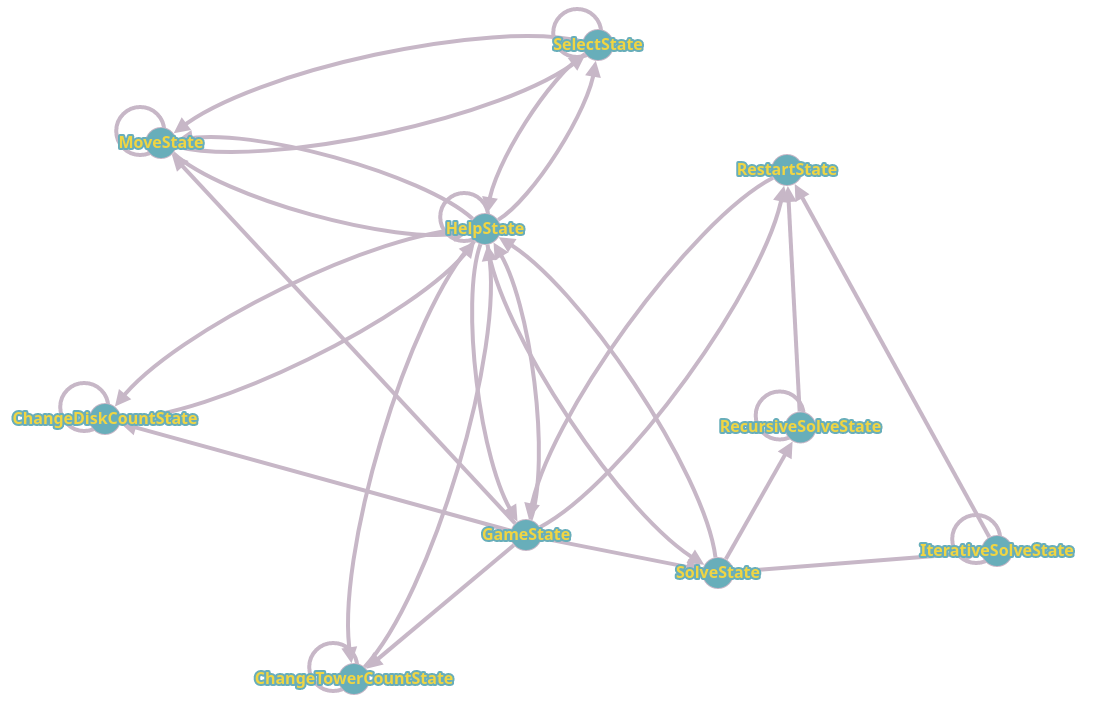
\includegraphics[width=\textwidth]{images/states.png}
		\caption{Граф состояний}
	\end{center}
\end{figure}

С помощью такой системы состояний очень легко расширять функционал программы.
Единственный минус такого способа борьбы со сложностью является написание
дополнительных классов. Такой минус не критичен, если система достаточно
большая.

Вся игра управляется с помощью главного состояния GameState. Из него можно
вызвать меню помощи (переход в состояние GameState $\rightarrow$ HelpState). Из
GameState можно перейти в состояние выбора автоматического решения (GameState
$\rightarrow$ SolveState), из него можно начать рекурсивное или итеративное
решение. После окончания автоматического решения происходит переход в состояние
RestartState. В любом режиме, кроме RecursiveSolveState и IterativeSolveState
можно попасть в режим HelpState, который может вернуть обратно в предыдущее
состояние, после прочтения меню помощи. Из GameState можно перейти в режим
ручного решения (GameState $\rightarrow$ MoveState). В этом режиме необходимо
выбрать диск, который игрок хочет перетащить. Если диск на башне отсутствует,
то мы остаёмся в режиме MoveState, иначе мы выбираем диск и переходим в
состоние выбора: куда переложить диск (MoveState $\rightarrow$ SelectState).
Если невозможно переложить диск (например диск большего размера не может быть
положен на диск меньшего размера), то мы остаёмся в режиме SelectState, иначе
мы перекладываем диск и возвращаемся в режим выбора диска для перекладывания
(SelectState $\rightarrow$ MoveState).

Важно понимать, при переходе из
состояния NameState$\rightarrow$NameState название состояния остаётся тем же,
но внутренние данные меняются, хотя в реализации всё иммутабельно (каждый раз
создаётся неизменяемый объект с новыми данными).

\begin{figure}[H]
	\begin{center}
		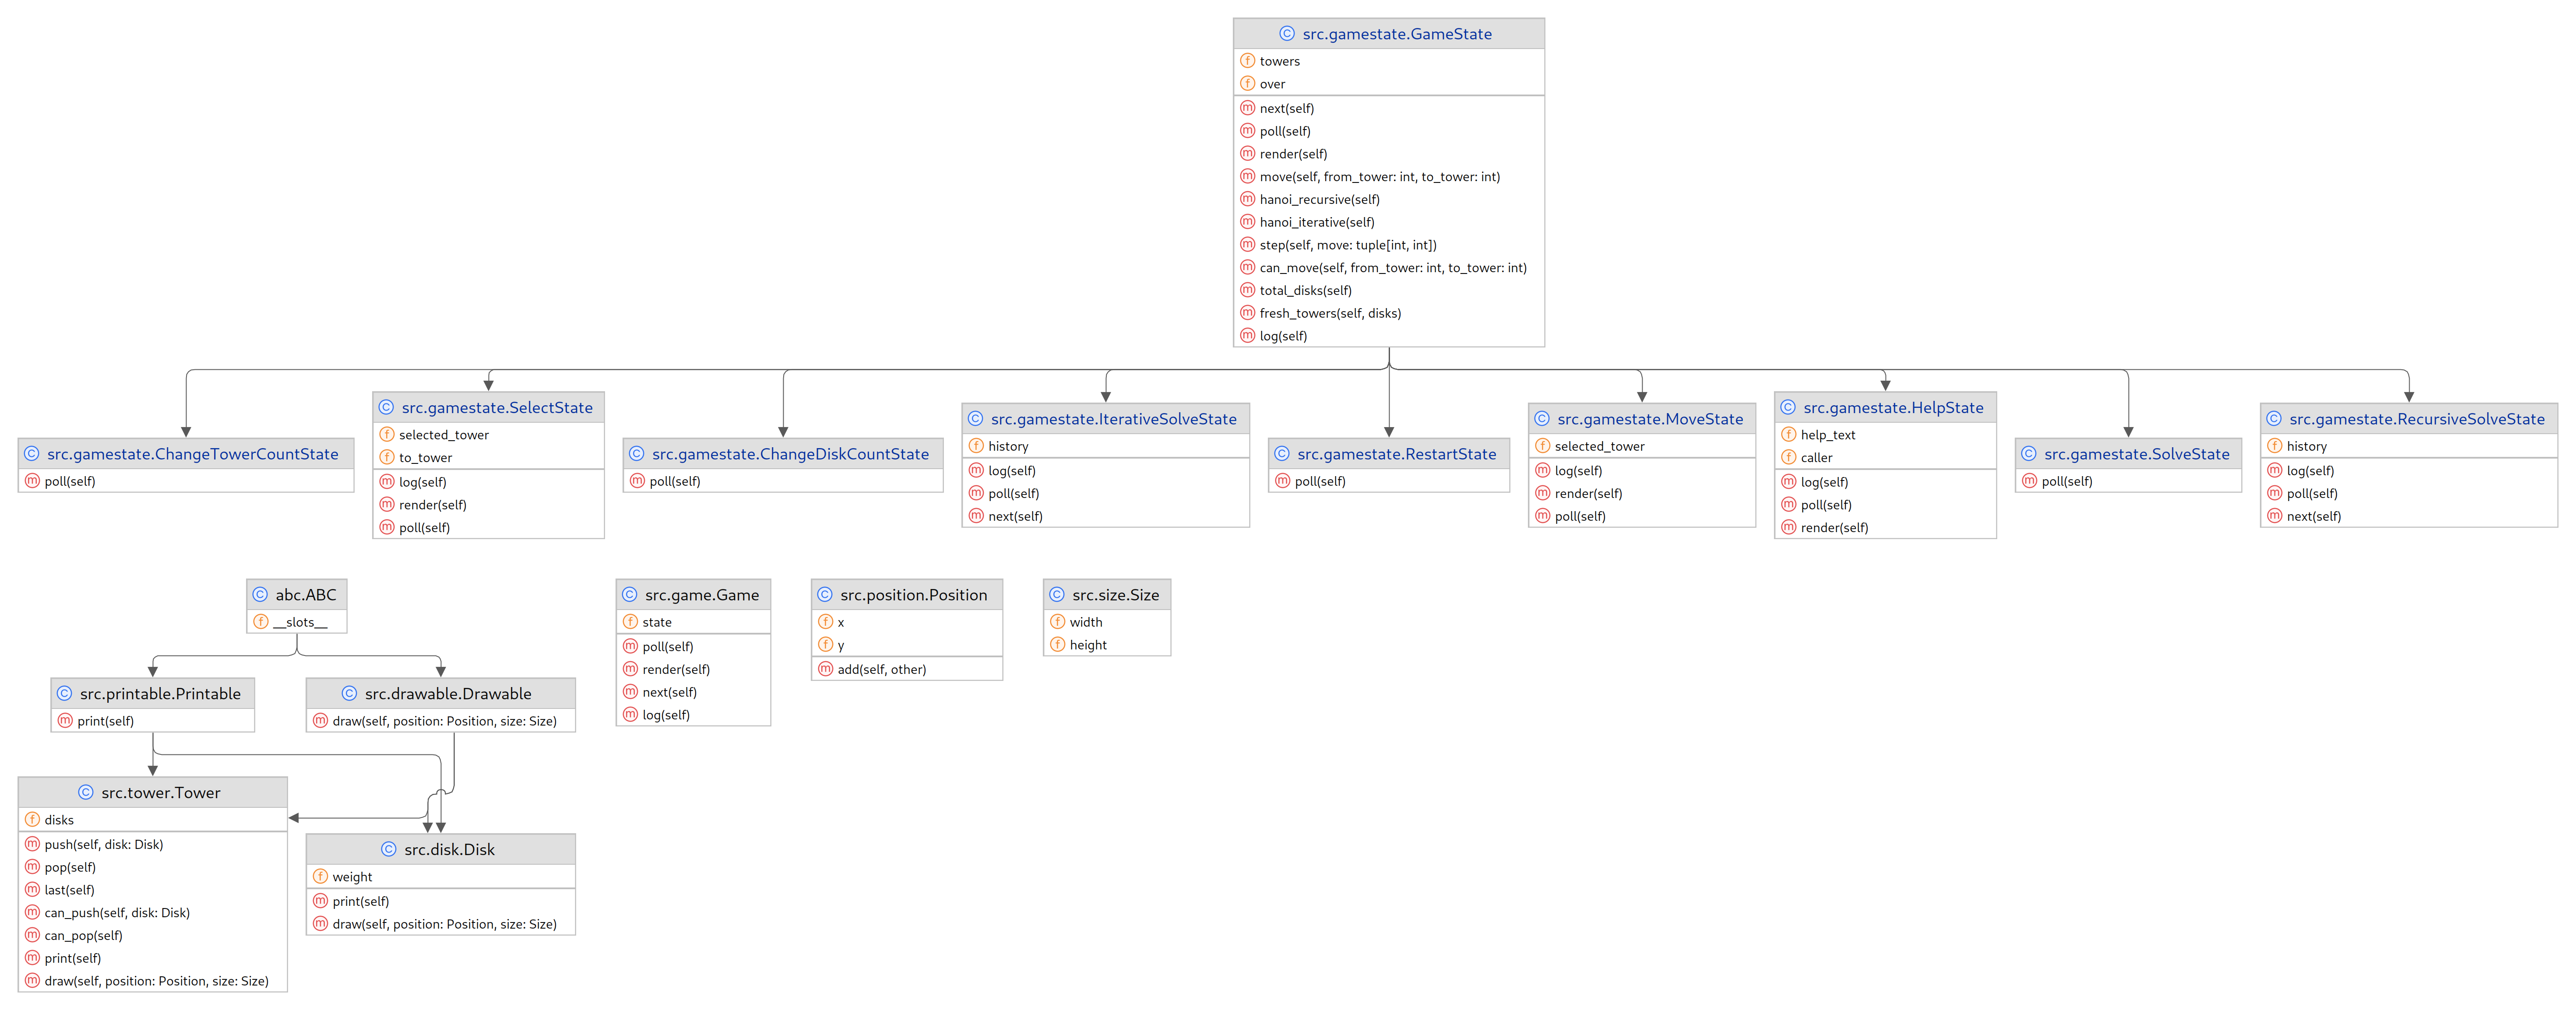
\includegraphics[width=\textwidth]{images/diagram.png}
		\caption{Диаграмма классов проекта}
	\end{center}
\end{figure}

Как и любая игра нашему проекту нужна инициализация данных (создание
первоначальных башен и дисков в правильном порядке). Инициализация игрового
``движка''. И главный цикл игры, в котором будет происходить в чётком порядке:

\begin{enumerate}
	\item Логгирования (log)
	\item Отрисовка (render)
	\item Отслеживание за нажатиями внутри игрового окна (poll)
	\item Изменение состояния игры (next)
\end{enumerate}

Важно отметить, что состоянии игры изменяется не только в методе next, но и,
конечно, вся магия мутации будет происходить внутри poll. Так как игрок будет
нажимать на клавиши клавиатуры, игра будет это воспринимать как собственное
изменение, например, переключение в другой режим игры.

Почти весь интерфейс состоит из прямоугольников разного цвета. Башни
располагаются симметрично и равноудалено относительно оси абсцисс. Дискам
задаётся ширина логарифмически. Высота всех дисков одинаковая. В интерфейсе
есть элементы текста, которые выводятся на экран, если программа находится в
состоянии HelpState.

\subsection{Рекурсивный алгоритм на Python}

\begin{code}
	\inputminted[breaklines=true, xleftmargin=1em, linenos, frame=single,
		framesep=10pt, fontsize=\footnotesize, firstline=119,
		lastline=137]{python}{../src/src/gamestate.py}
	\caption{Одна из рекурсивных реализаций алгоритма решения задачи о Ханойской
		башне}
\end{code}


\subsection{Итеративный алгоритм на Python}

\begin{code}
	\inputminted[breaklines=true, xleftmargin=1em, linenos, frame=single,
		framesep=10pt, fontsize=\footnotesize, firstline=139,
		lastline=168]{python}{../src/src/gamestate.py}
	\caption{Одна из итеративных реализаций алгоритма решения задачи о Ханойской
		башне}
\end{code}

\subsection{Тестирование библиотеки}

Программа-игра может автоматически решать задачу о Ханойской башне. Существует
режим ручной игры, где игрок перетаскивает диски по правилам игры. 

В ходе тестирования были проверены все режимы:

\begin{itemize}
  \item Режим ручной игры
  \item Автоматический режим решения: рекурсивный и итеративный
  \item Режим изменения количества дисков
  \item Режим изменения количества башен
\end{itemize}

Во всех режимах не было обнаружено каких-либо ошибок в работе программы.

В ходе выполнения работы были написаны юнит-тесты для библиотеки классов.
Было протестировано перемещение дисков между башнями: нельзя допустить, чтобы
диск был помещён не по-правилам пазла.

Юнит-тесты дают точно понять, не нарушили мы главные библиотечные вызовы:
перемещение дисков между башнями и помещение диска внутрь башни.

Игра разрешает играть с как минимум 1 диском.

Всё тестирование проходило на версии \verb|Python 3.10.8|.

Во время ручного тестирования на ОС Linux ошибок выявлено не было.
На машине с ОС MS Windows была выявлена ошибка разрешения экрана.
Чтобы решить данную проблему пришлось изменять настройки масштабирования экрана.
Масштабирование экрана должно быть 100\%.

Если количество дисков равно 0, то задача решена, но в интерфейсе нет такой
возможности. При количестве дисков $\le 1$ задача успешно решается с
помощью алгоритма.

У алгоритмов не ограничений по количеству дисков. При достаточно большом
количестве ($>25$) программа может достаточно долго выполняться и занять всю
оперативную память компьютера.

Игра ведёт журнал (логгирование) в стандартный выход (терминал), в котором есть
следующая информация: текущее состояние игры (NameState), состояние башен и
дисков. В режиме HelpState дублируется текст, выведенный на экран, в лог
журнала. В режиме MoveState логгируется текущее положение курсора (текущая
башня под курсором). В режиме SelectState логгируется положение курсора из
MoveState и положение курсора куда мы хотим сделать ход. В режиме решения
выводится история ходов, которые надо совершить.

\subsection{Пример работы программы}

\begin{figure}[H]
	\begin{center}
		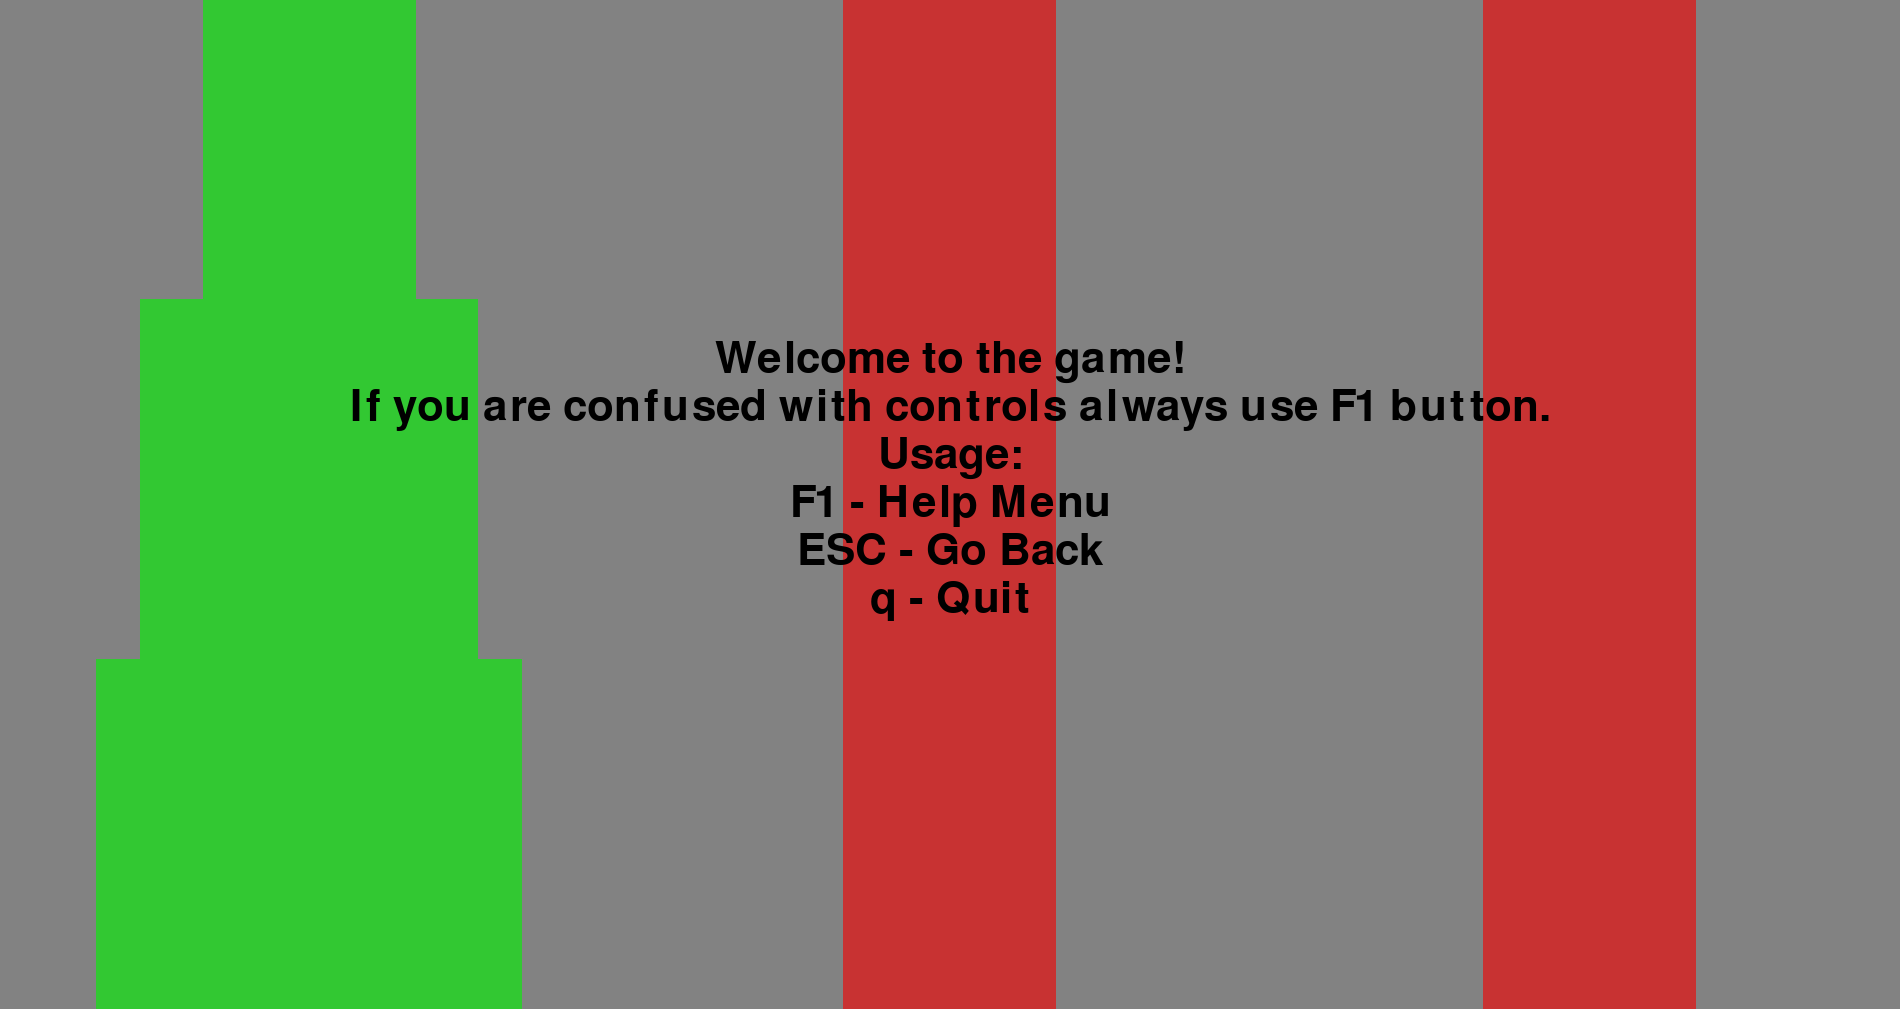
\includegraphics[width=\textwidth]{images/main_menu.png}
		\caption{Главное меню игры}
	\end{center}
\end{figure}
\begin{figure}[H]
	\begin{center}
		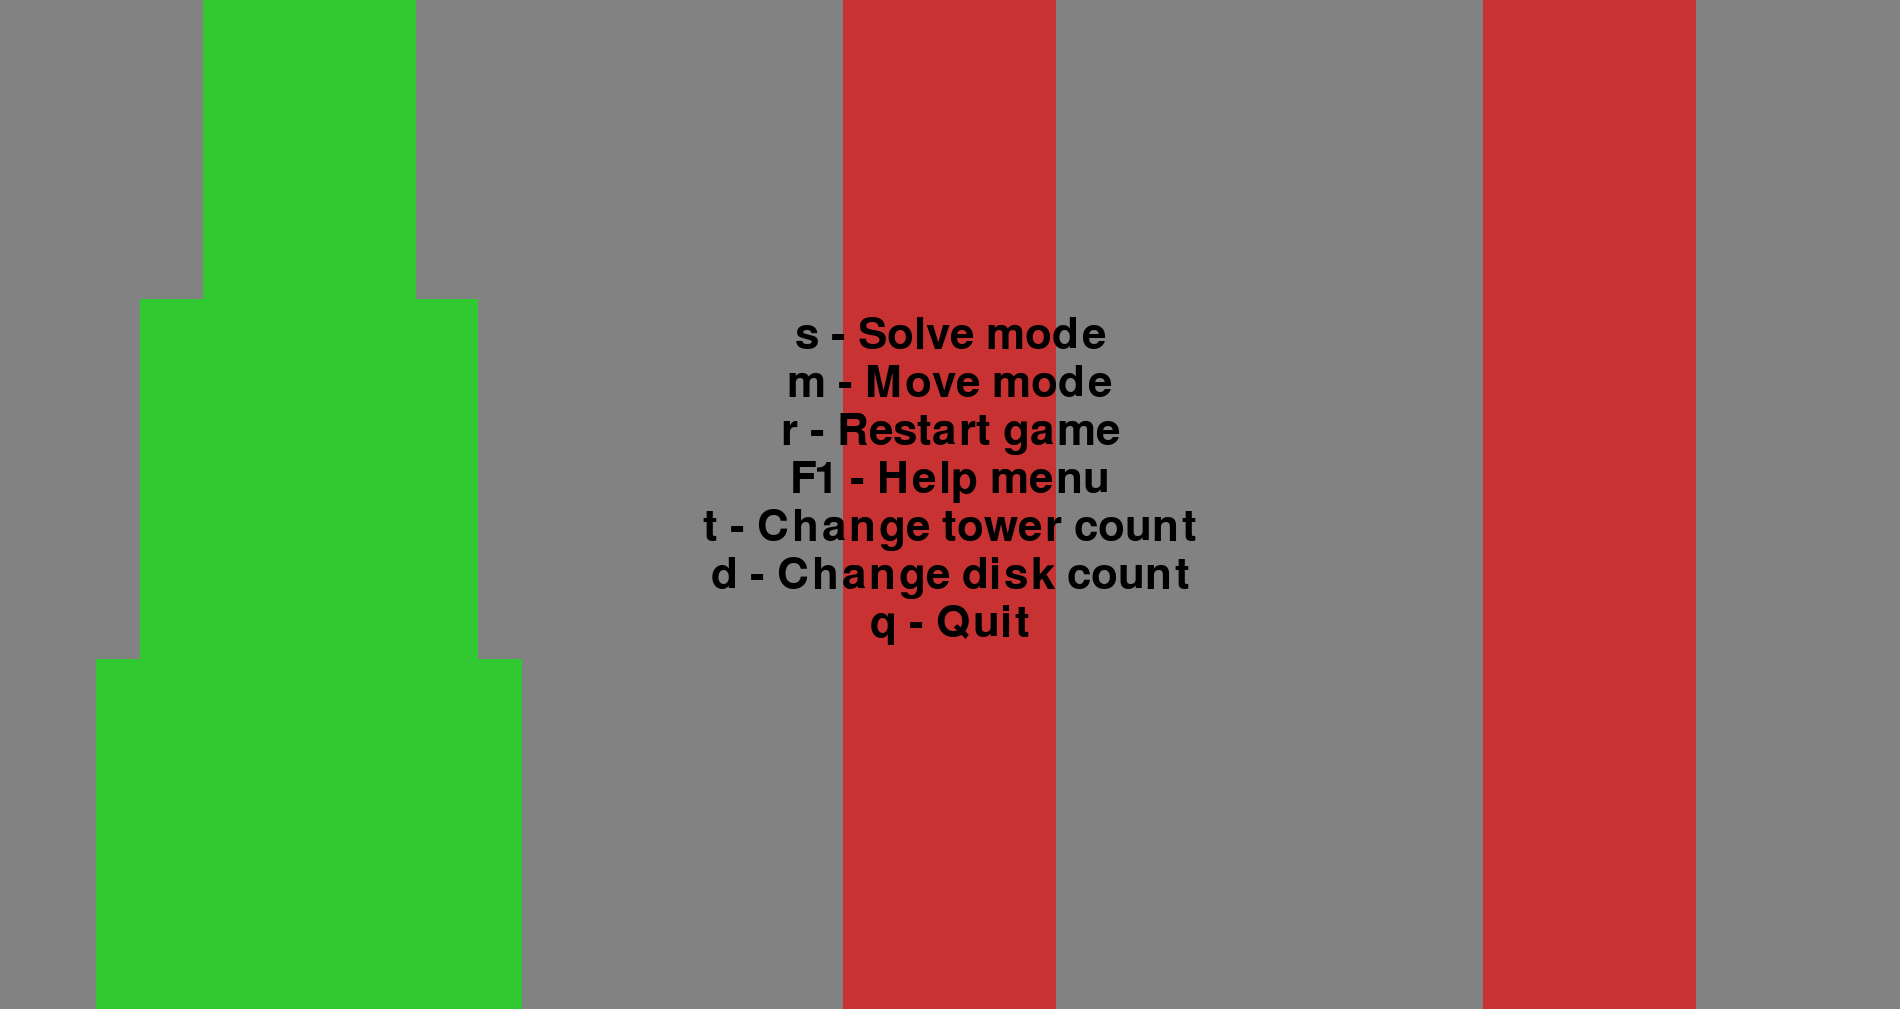
\includegraphics[width=\textwidth]{images/main_help.png}
		\caption{Главное меню помощи. управление}
	\end{center}
\end{figure}
\begin{figure}[H]
	\begin{center}
		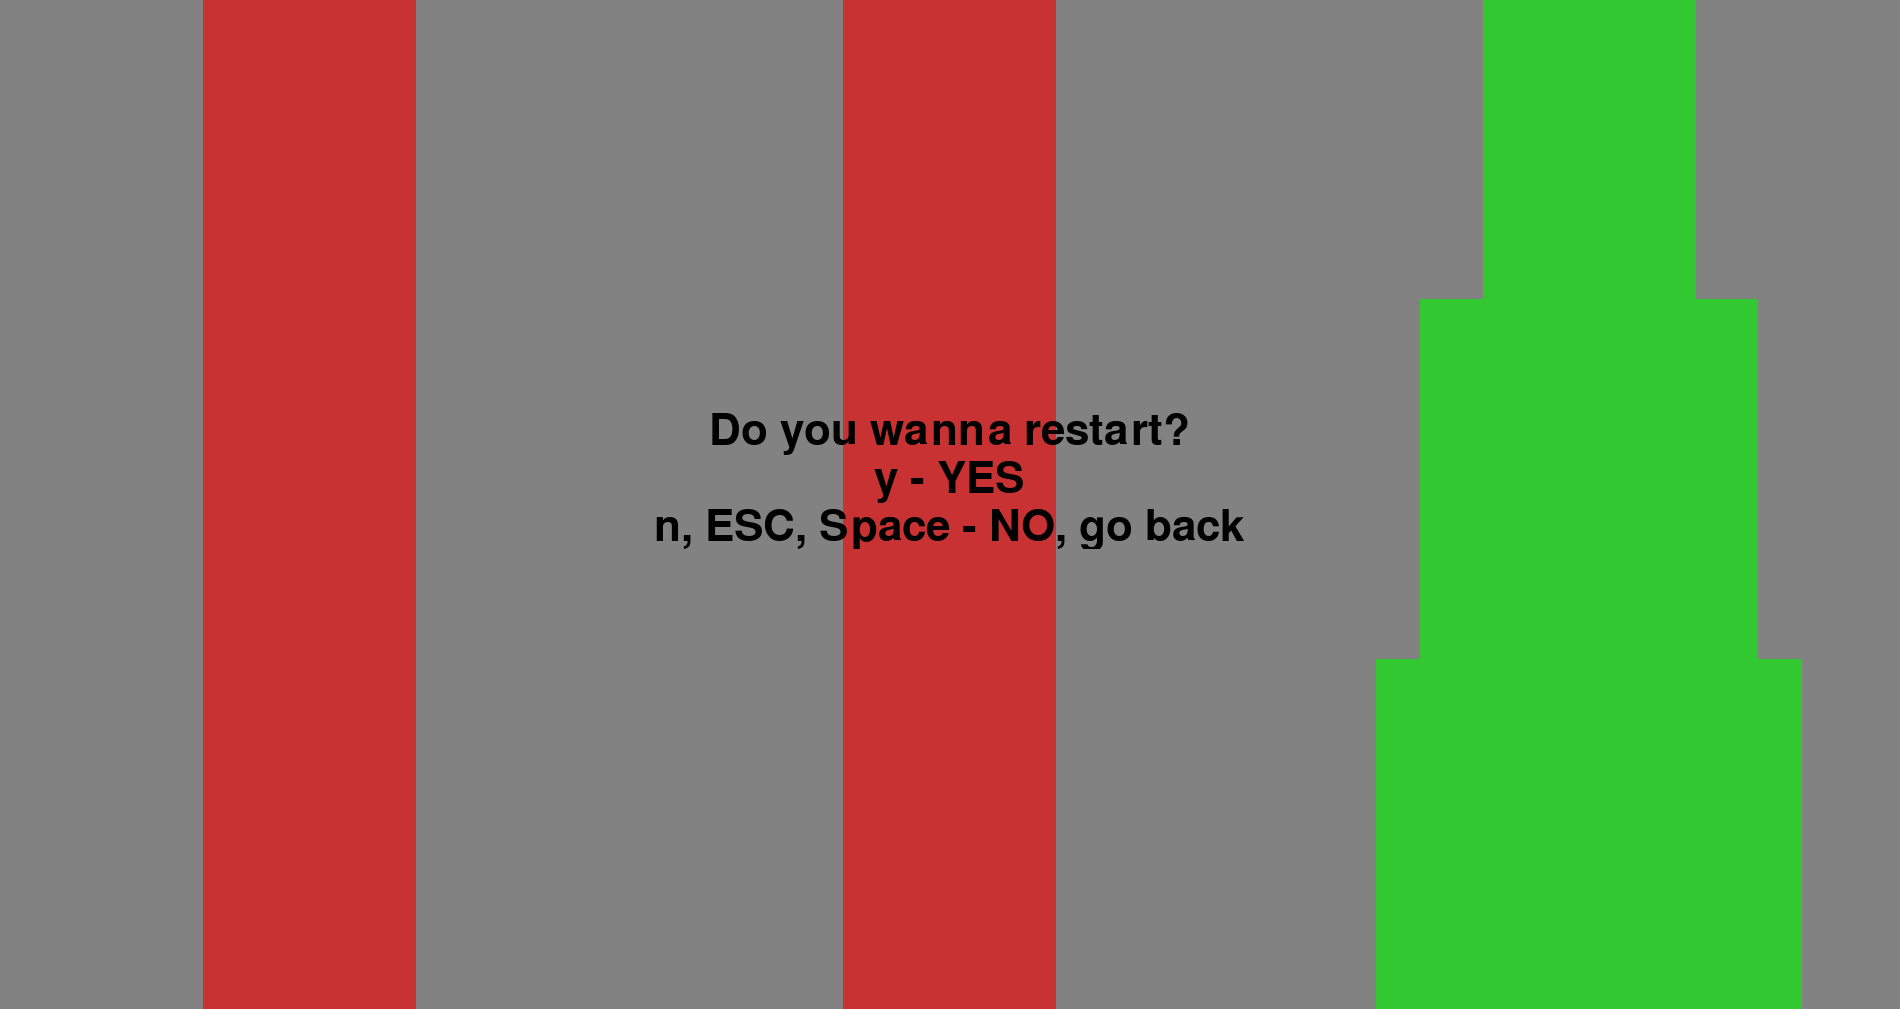
\includegraphics[width=\textwidth]{images/finish.png}
		\caption{В конце авто-решения головоломки можно перезапустить игру}
	\end{center}
\end{figure}
\begin{figure}[H]
	\begin{center}
		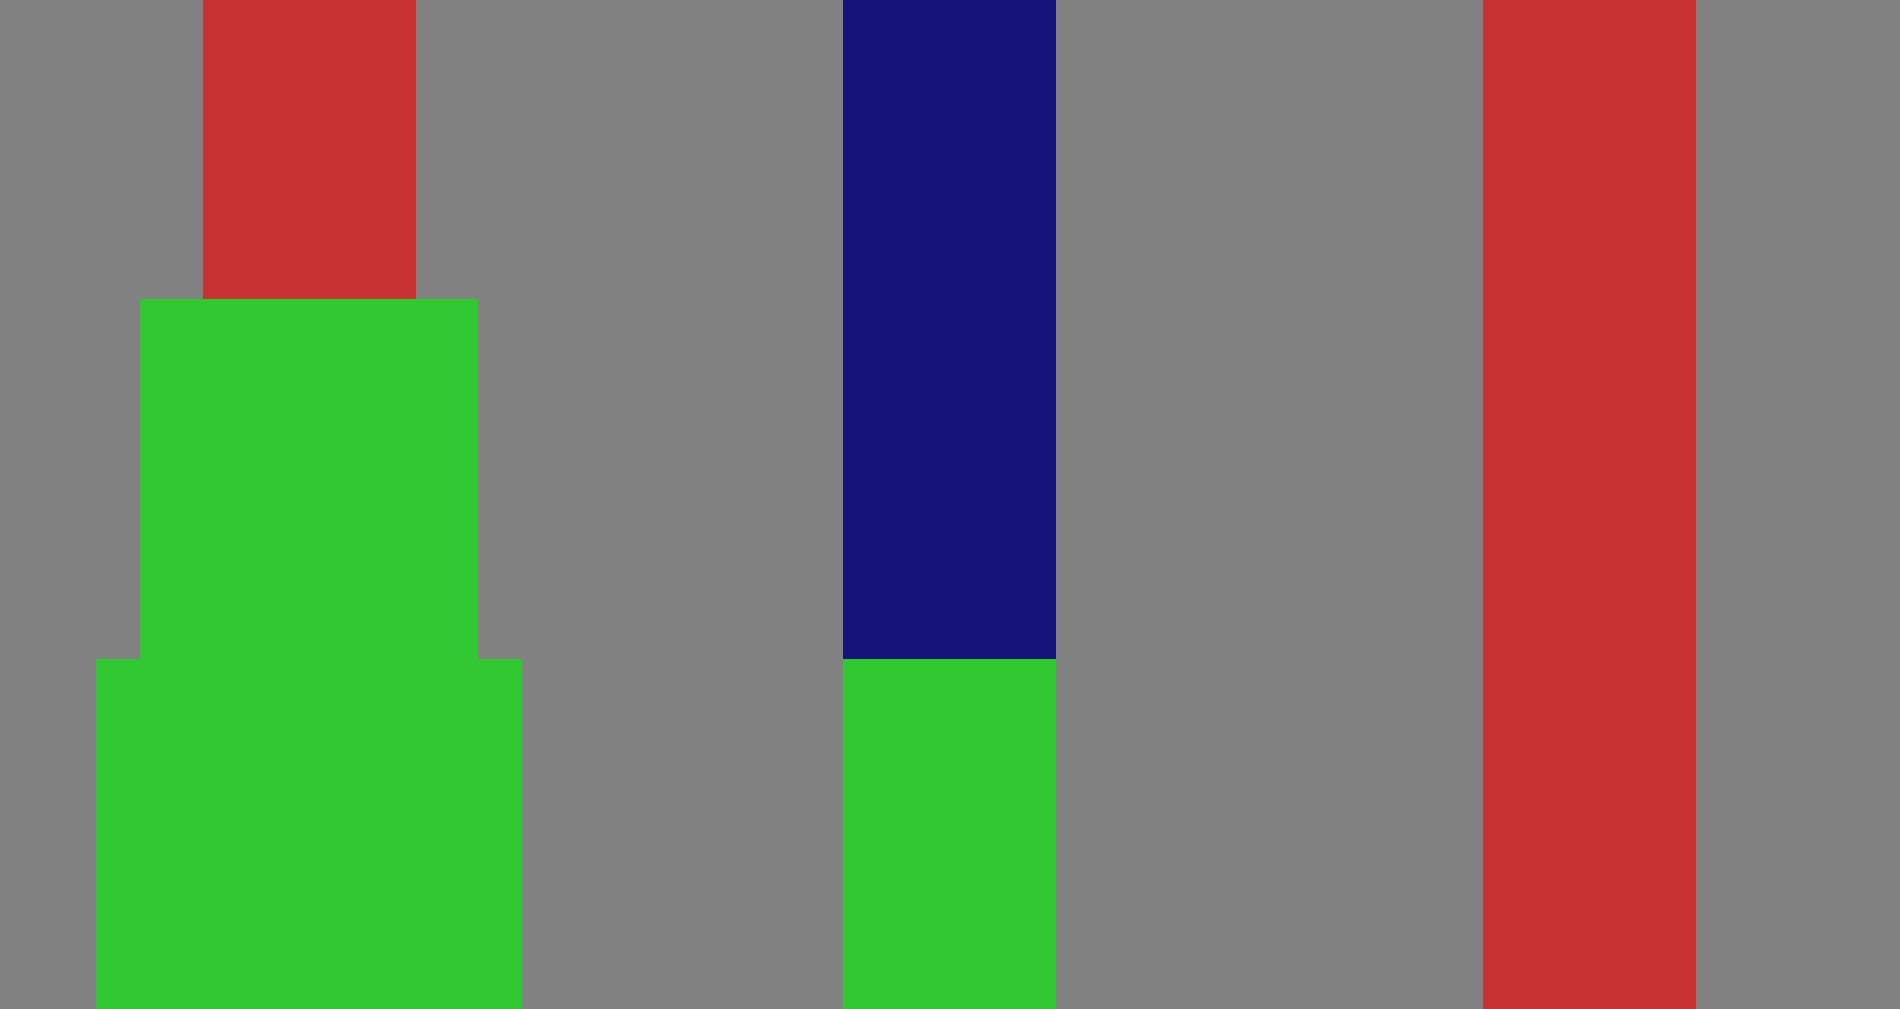
\includegraphics[width=\textwidth]{images/move_mode.png}
		\caption{Меню передвижения курсора для взятия диска}
	\end{center}
\end{figure}
\begin{figure}[H]
	\begin{center}
		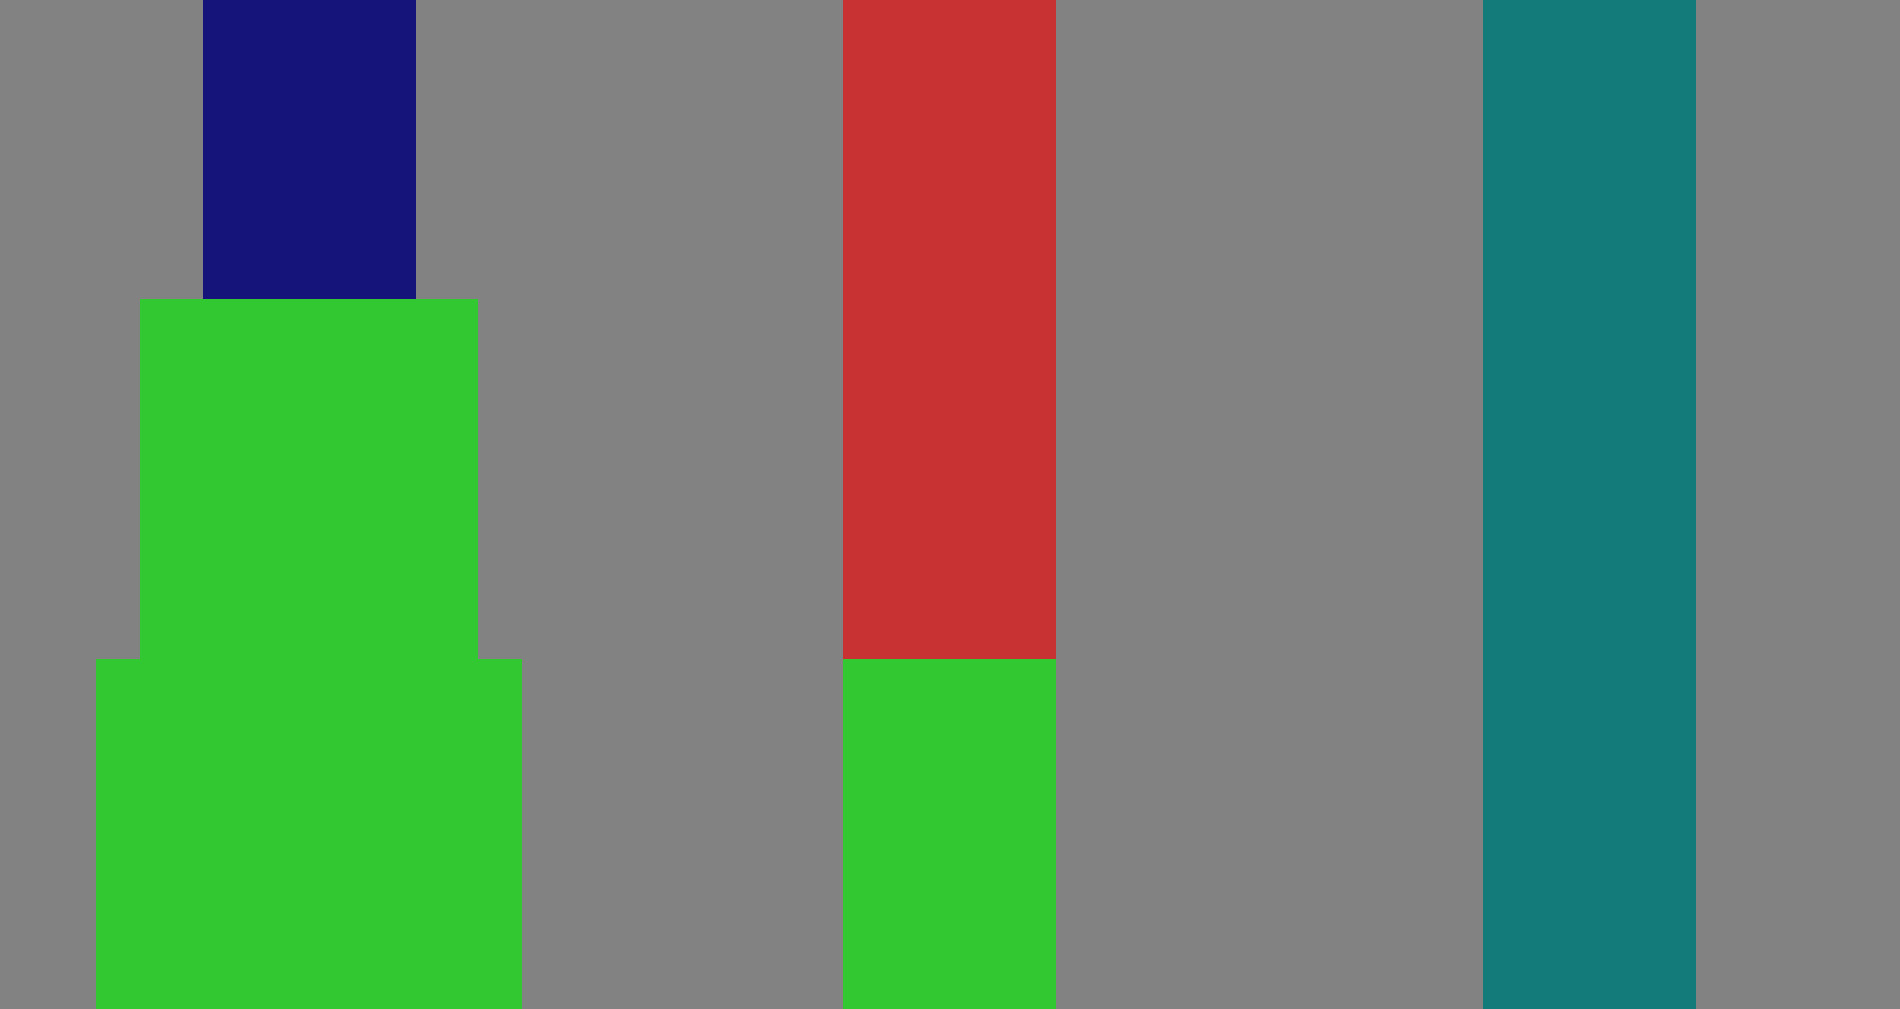
\includegraphics[width=\textwidth]{images/select_mode.png}
		\caption{Меню выбора нового положения для выбранного диска}
	\end{center}
\end{figure}
\begin{figure}[H]
	\begin{center}
		
\includegraphics[width=\textwidth]{images/many_disks.png}
		\caption{Возможно увеличить или уменьшить количество дисков}
	\end{center}
\end{figure}
\begin{figure}[H]
	\begin{center}
		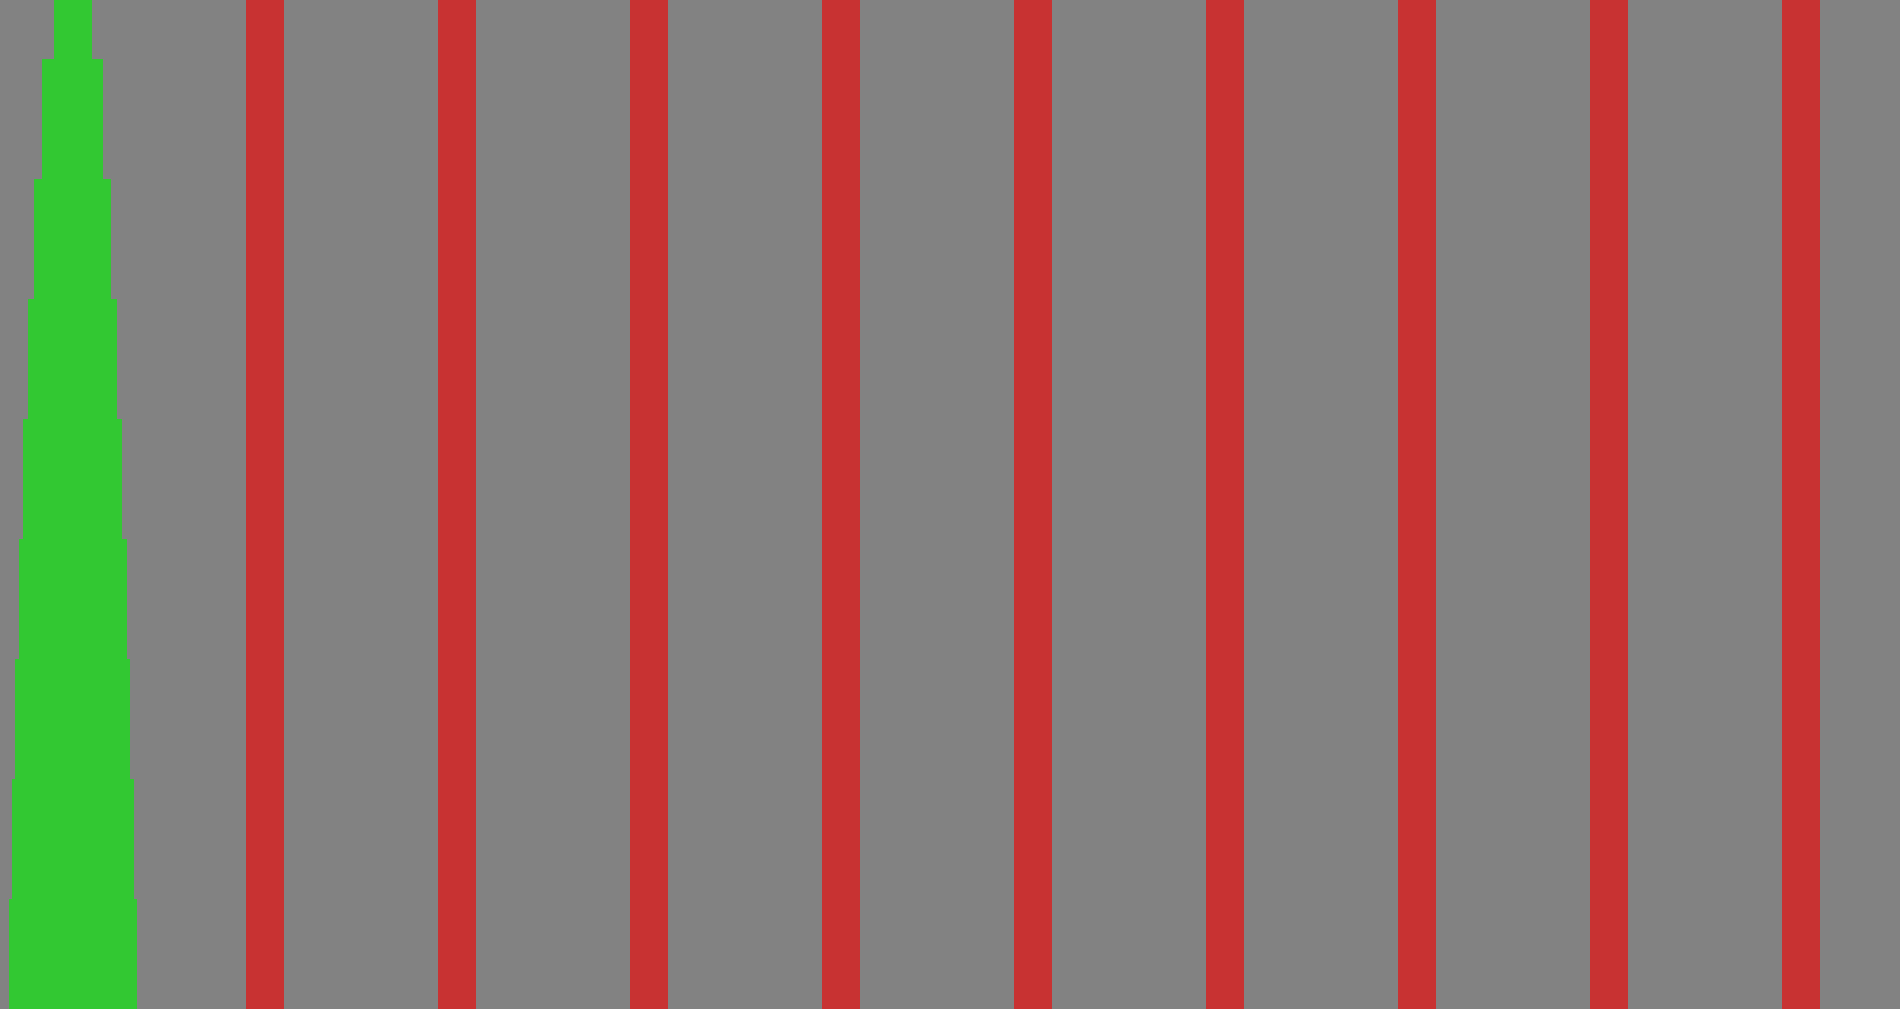
\includegraphics[width=\textwidth]{images/many_towers.png}
		\caption{Возможно увеличить или уменьшить количество башен}
	\end{center}
\end{figure}

\section*{Заключение}
Рассмотрели теоретическую информацию о рекурсивном и итеративном алгоритме. В
данной реализации итеративного алгоритма видно, что он абсолютно идентичен по
ходам с рекурсивным алгоритмом. Итеративный алгоритм сложнее в реализации, для
него требуется знание о том, можно ли сделать легальный ход в обе стороны.

Реализовали полноценную игру, рекурсивный и итеративные алгоритмы решения
задачи о Ханойской башне. Так же пользователю дана возможность решить задачу
самостоятельно. Весь код можно найти по данному адресу:
\url{https://github.com/andreymlv/tstu-computation-theory}
\addcontentsline{toc}{section}{Заключение}
